\documentclass[12pt]{article}
\usepackage{geometry}                % See geometry.pdf to learn the layout options. There are lots.
\geometry{letterpaper}                   % ... or a4paper or a5paper or ... 
%\geometry{landscape}                % Activate for for rotated page geometry
\usepackage[parfill]{parskip}    % Activate to begin paragraphs with an empty line rather than an indent
\usepackage{daves,fancyhdr,natbib,graphicx,dcolumn,amsmath,lastpage,url}
\usepackage{amsmath,amssymb,epstopdf,longtable}
\usepackage[final]{pdfpages}
\DeclareGraphicsRule{.tif}{png}{.png}{`convert #1 `dirname #1`/`basename #1 .tif`.png}
\pagestyle{fancy}
\lhead{CE 3354 -- Engineering Hydrology}
\rhead{SUMMER 2025}
\lfoot{ES7}
\cfoot{}
\rfoot{Page \thepage\ of \pageref{LastPage}}
\renewcommand\headrulewidth{0pt}



\begin{document}
\begin{center}
{\textbf{{ CE 3354 Engineering Hydrology} \\ {Exercise Set 7}}}
\end{center}

\section*{\small{Exercises}}
\begin{enumerate}

\item Figure \ref{fig:OklahomaData} The following data represent gage height and annual peak discharge for some gaging station in Oklahoma.  The stage is in feet and the discharge is in cubic feet per second.  The data are sequential from 1923 through 1971.

\begin{figure}[h!] %  figure placement: here, top, bottom, or page
   \centering
   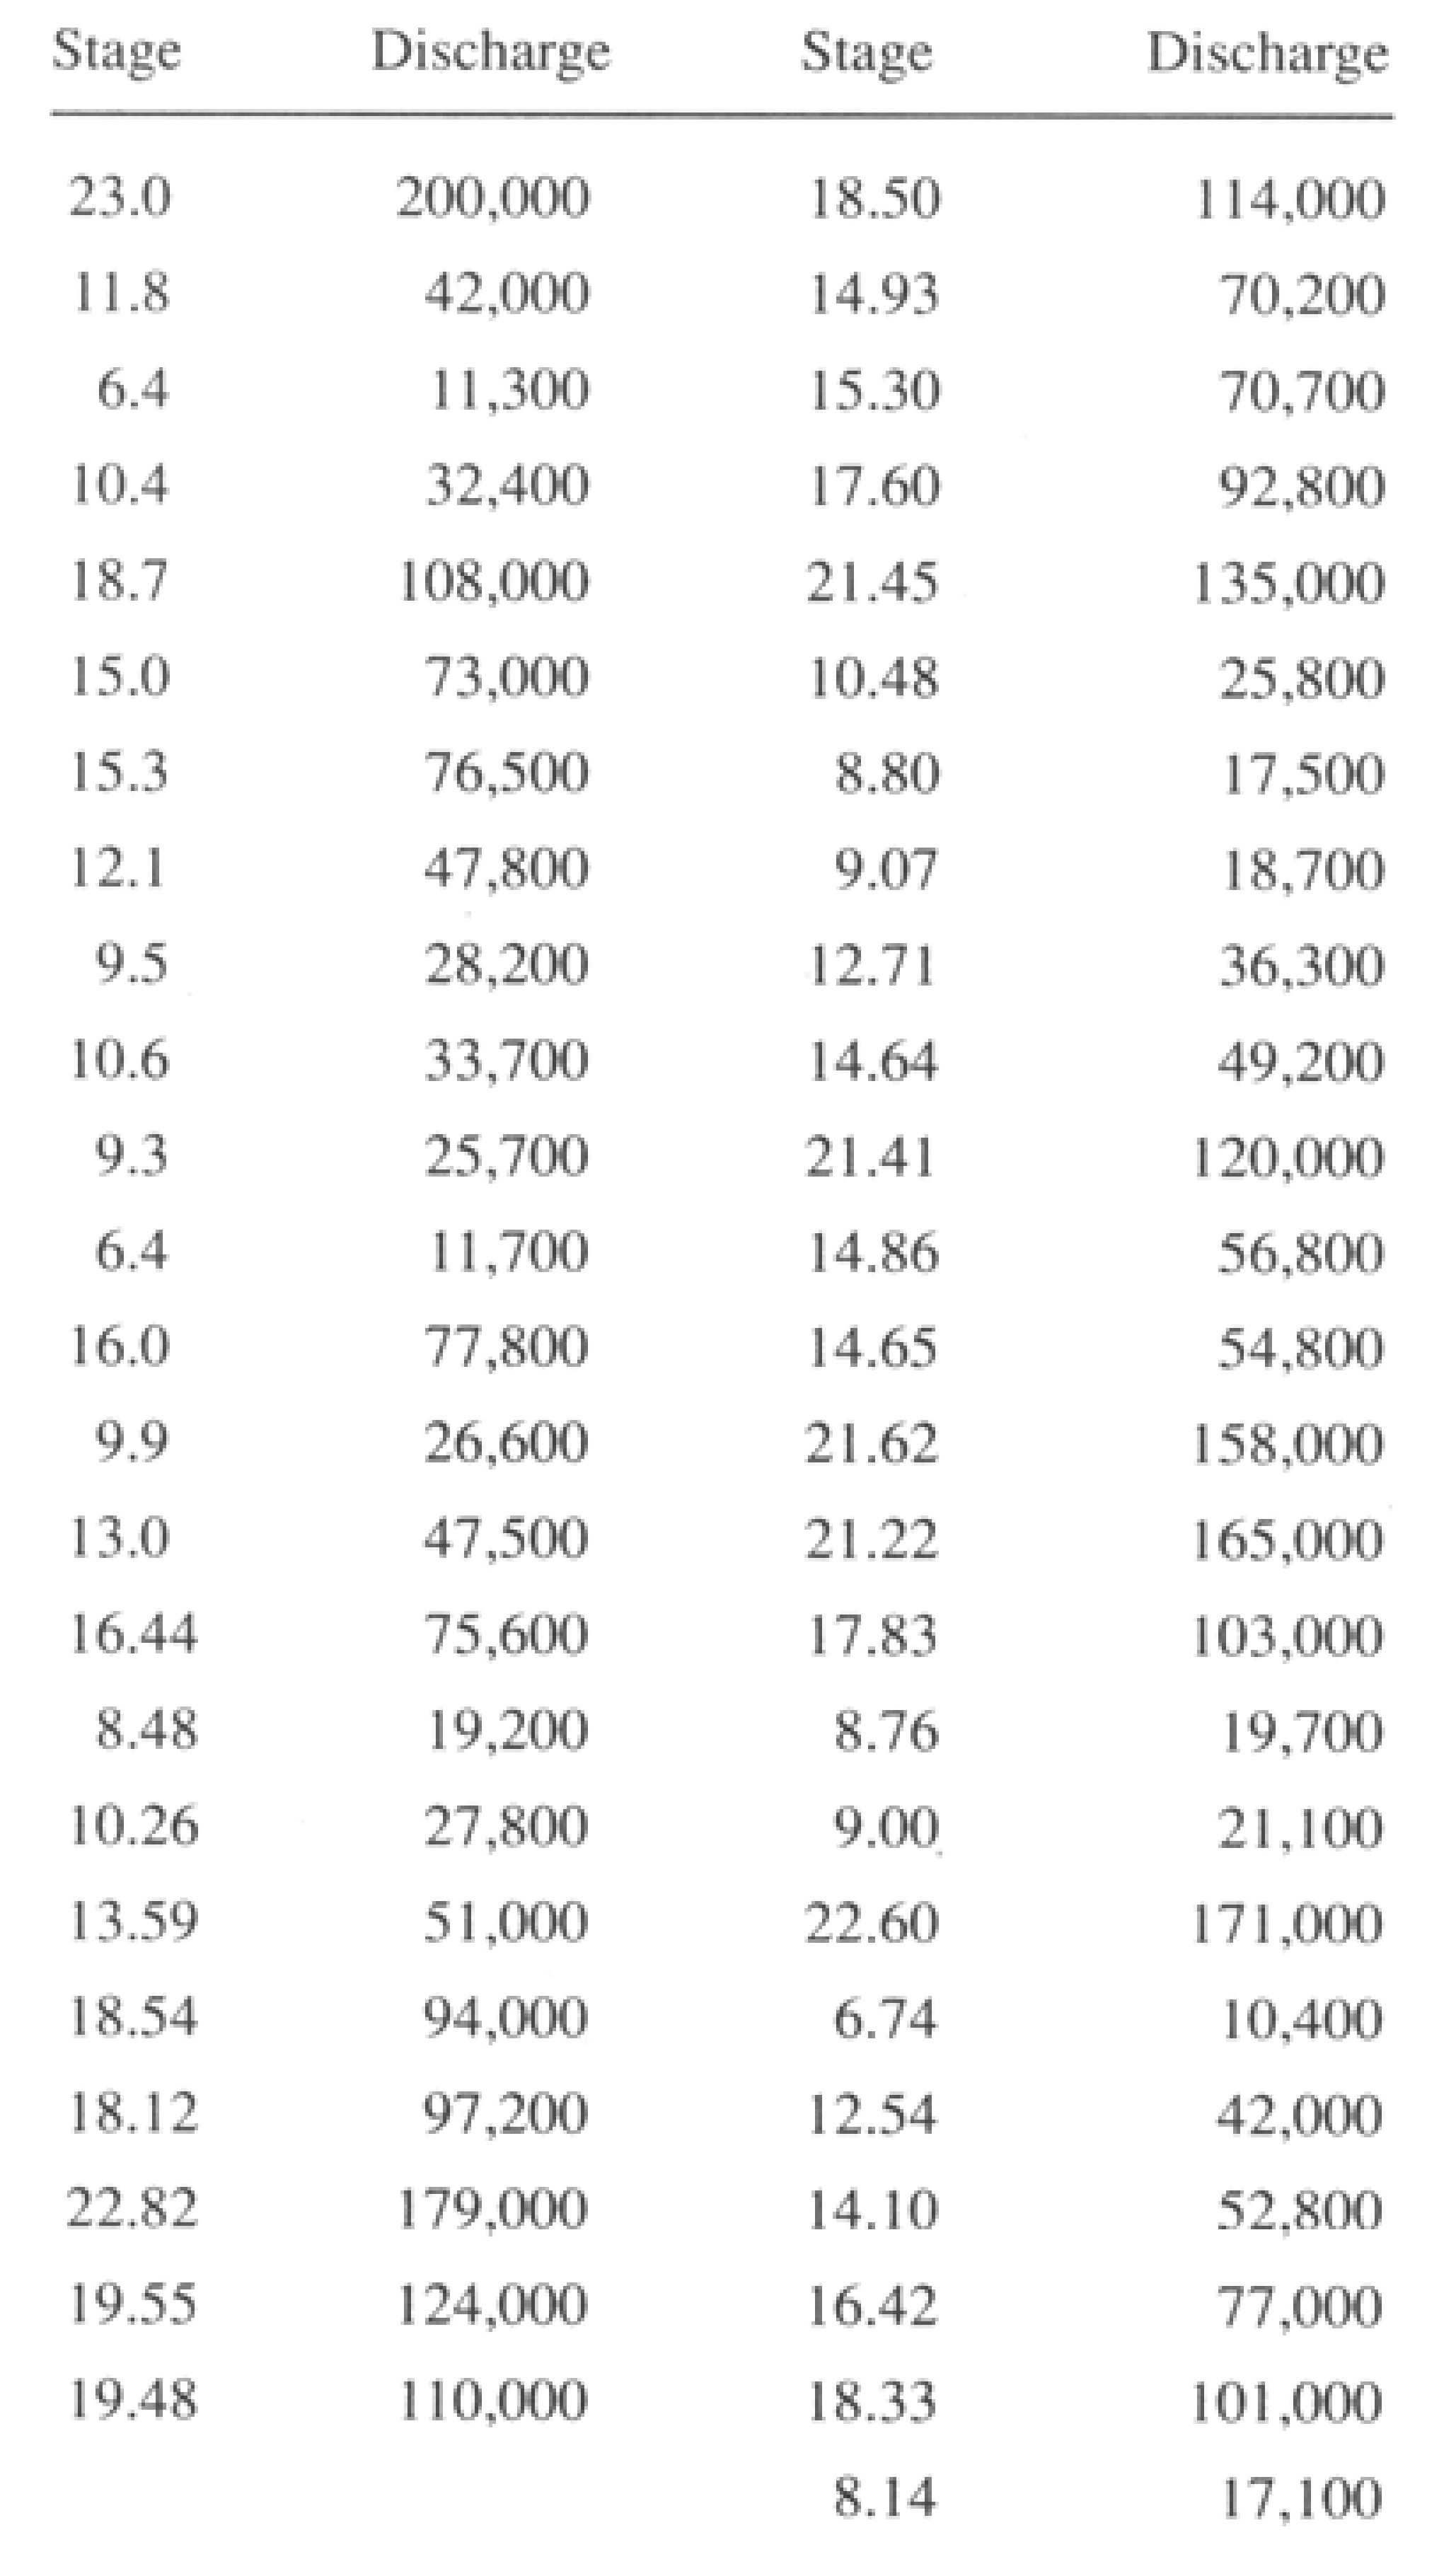
\includegraphics[height=7in]{OklahomaData.jpg} 
   \caption{Data from Oklahoma Gaging Station}
   \label{fig:OklahomaData}
\end{figure}

Use the data to:
\begin{enumerate}
\item Plot year versus stage ( x-axis is year).
\item Plot year versus discharge ( x-axis is year).
\item Plot the discharge versus stage.
\item Using the Weibull plotting position formula, determine the distribution parameters that fit the data for a log-normal distribution.
\item Using the Weibull plotting position formula, determine the distribution parameters that fit the data for a Gumbell distribution.
\item Using the Weibull plotting position formula, determine the distribution parameters that fit the data for a Gamma distribution.
\item Estimate the discharge associated with a 25-percent chance exceedence probability (i.e. the value that is equal to or exceeded with a 1 in 4 chance).
\item A resident claims that in the early 1900?s a flood corresponding to a stage of 30 feet occurred at the gage location.  Estimate the exceedence probability (return period) of the flow associated with this event.
\end{enumerate}
\clearpage
\textbf{Solution(s) attached next page}

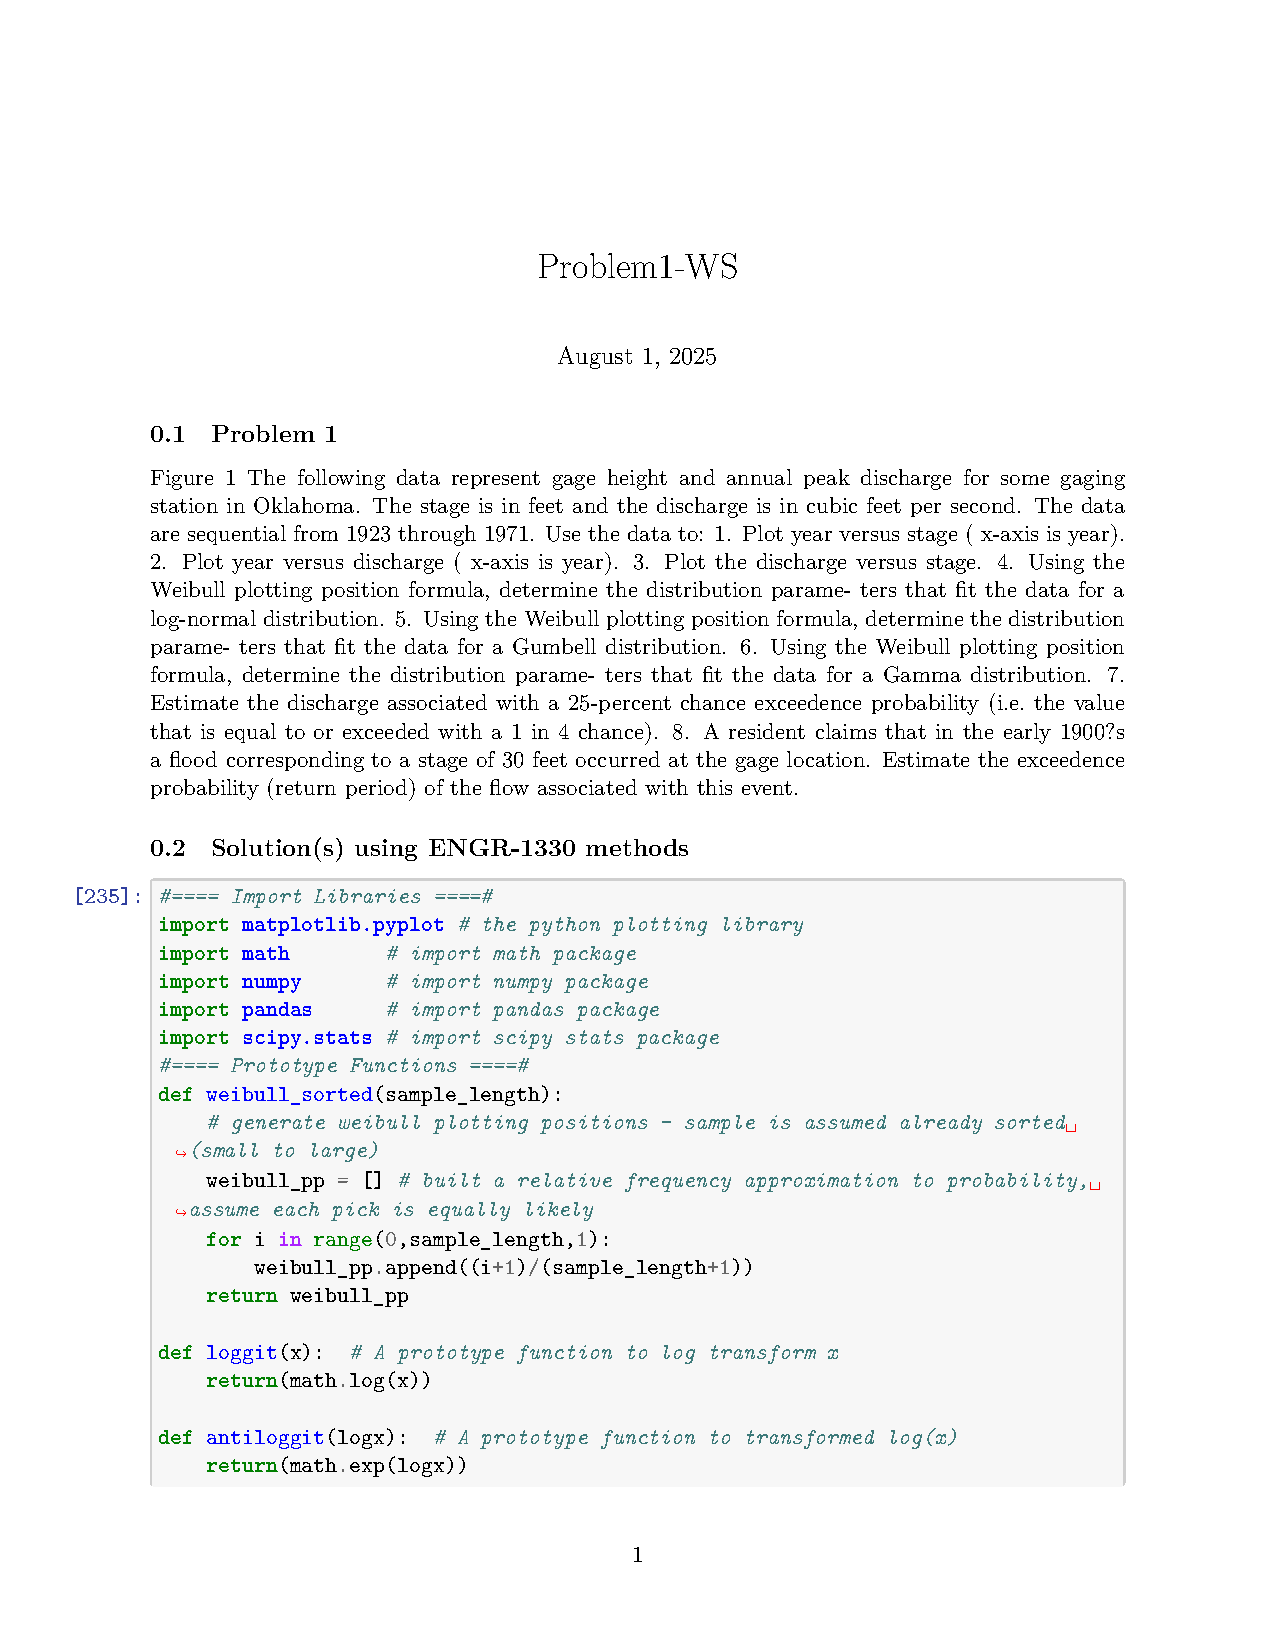
\includepdf[pages=-]{Problem1-WS.pdf}


\item Use the Oklahoma data you just prepared and analyze using the Bulletin 17C procedure (using the HEC-SSP software tool - use station skew option).

\textbf{Solution(s) below}
\begin{figure}[h!] %  figure placement: here, top, bottom, or page
   \centering
   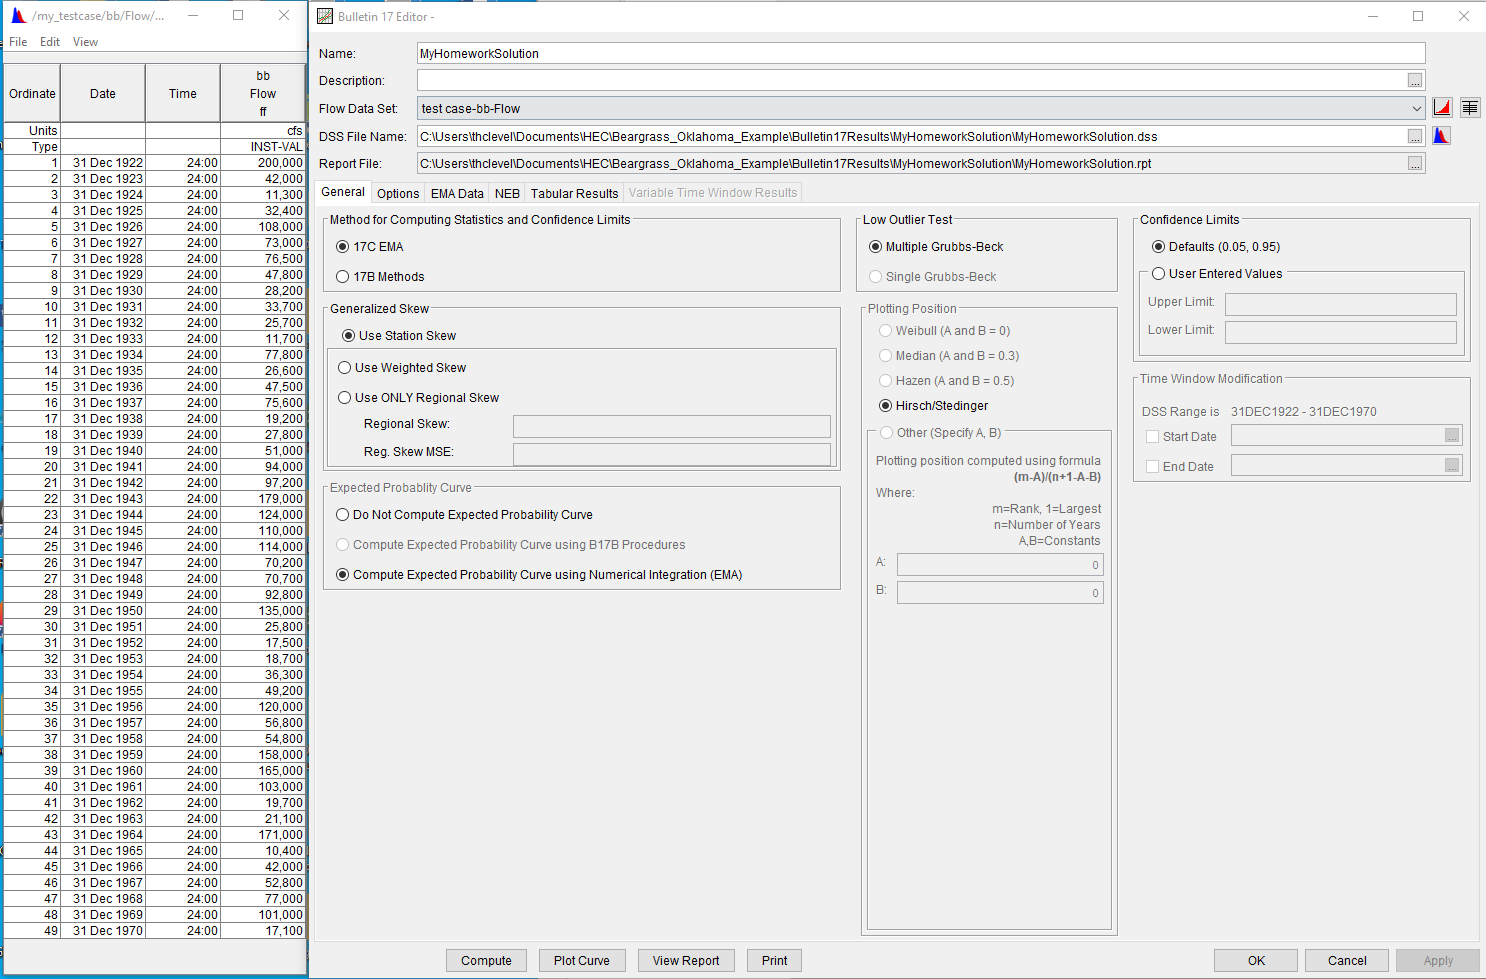
\includegraphics[width=7in]{HEC-SSP-interface.png} 
   \caption{Interface and Data from Oklahoma Gaging Station}
   \label{fig:HEC-SSP-interface}
\end{figure}

\begin{figure}[h!] %  figure placement: here, top, bottom, or page
   \centering
   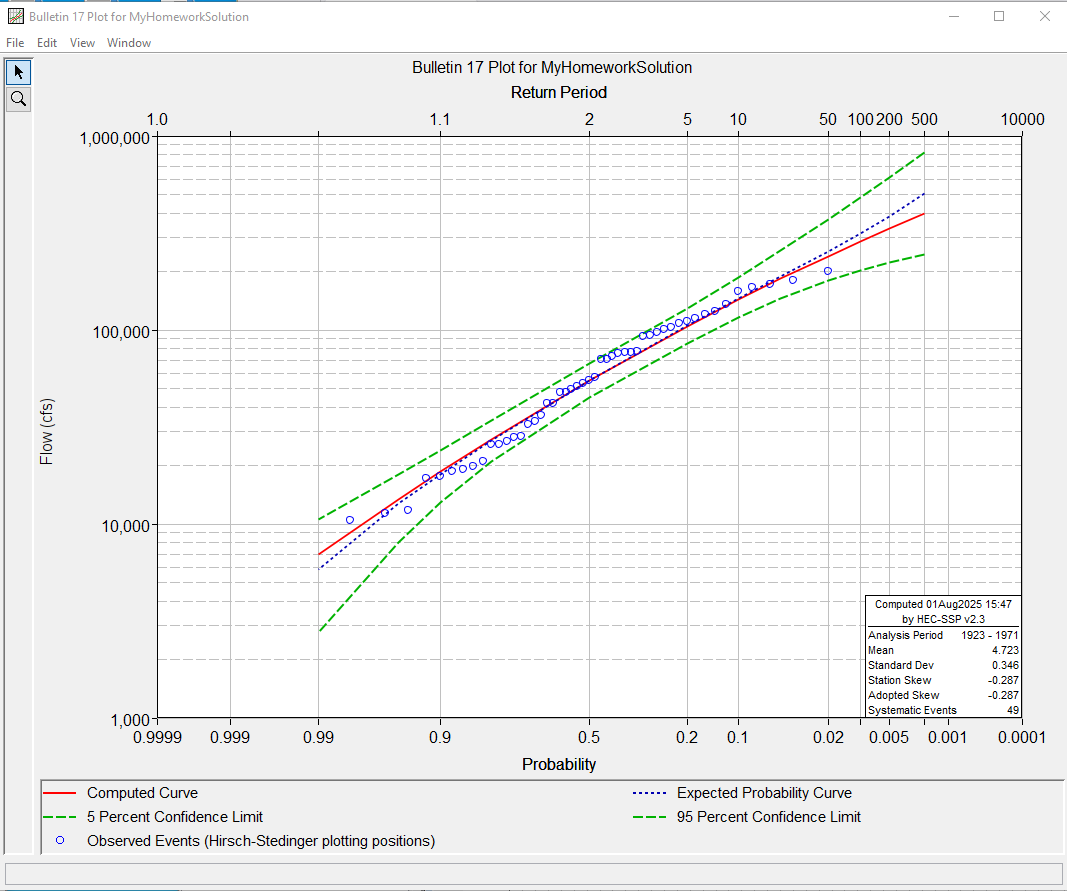
\includegraphics[width=7in]{HEC-SSP-plot.png} 
   \caption{Probability Plot from Oklahoma Gaging Station}
   \label{fig:HEC-SSP-interface}
\end{figure}

\begin{figure}[h!] %  figure placement: here, top, bottom, or page
   \centering
   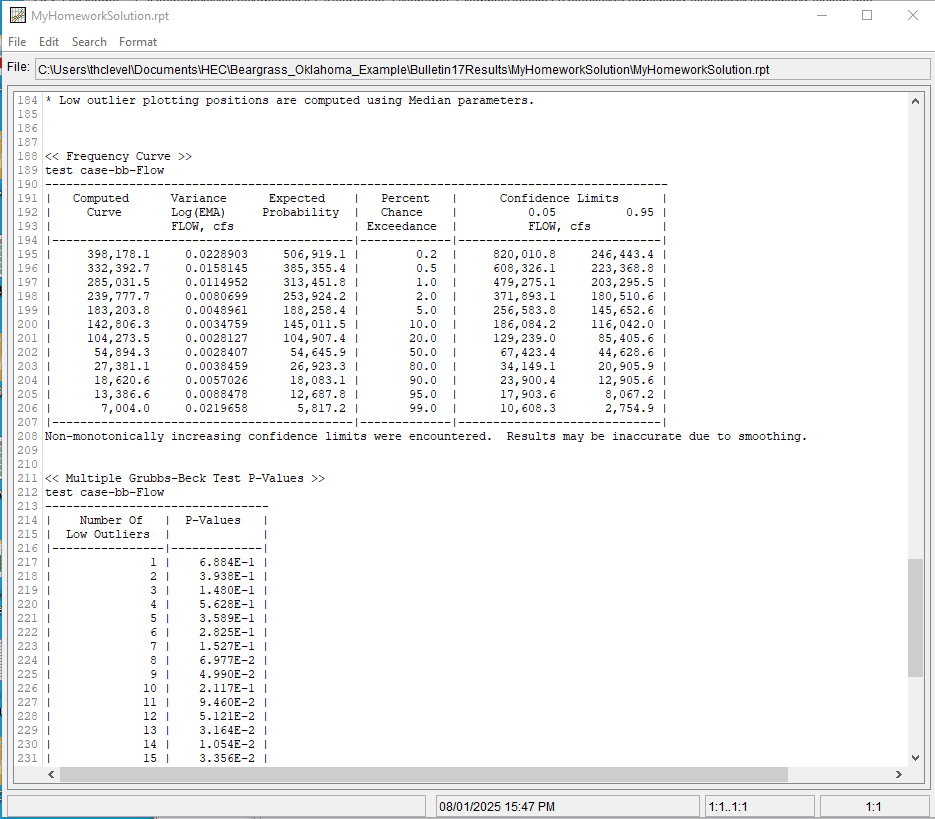
\includegraphics[width=7in]{HEC-SSP-tabulation.png} 
   \caption{Probability Tabulation from Oklahoma Gaging Station}
   \label{fig:HEC-SSP-interface}
\end{figure}

The 0.25 AEP (4-year ARI) value falls between 104,273 CFS at 0.20 AEP and 54,894 CFS at 0.50 AEP.  Logarithmic interpolation produces an estimate of 89,189 CFS which is close to our homebrew result of 91,615 CFS for the same AEP value.

\clearpage

\item  Locate USGS Station 08144800 Brady Creek near Eden, TX. and analyze the historical peaks using the Bulletin 17C procedures (use the PeakFQ software tool use station skew option).  Determine the median discharge predicted for this station by PeakFQ.  Also determine the discharge per square mile of contributing drainage area.\footnote{Download the annual peaks from NWIS in the tab-delimited format for use in peakFQ; The example in the instructor notes is this particular site.}

\textbf{Solution(s) below}
\begin{figure}[h!] %  figure placement: here, top, bottom, or page
   \centering
   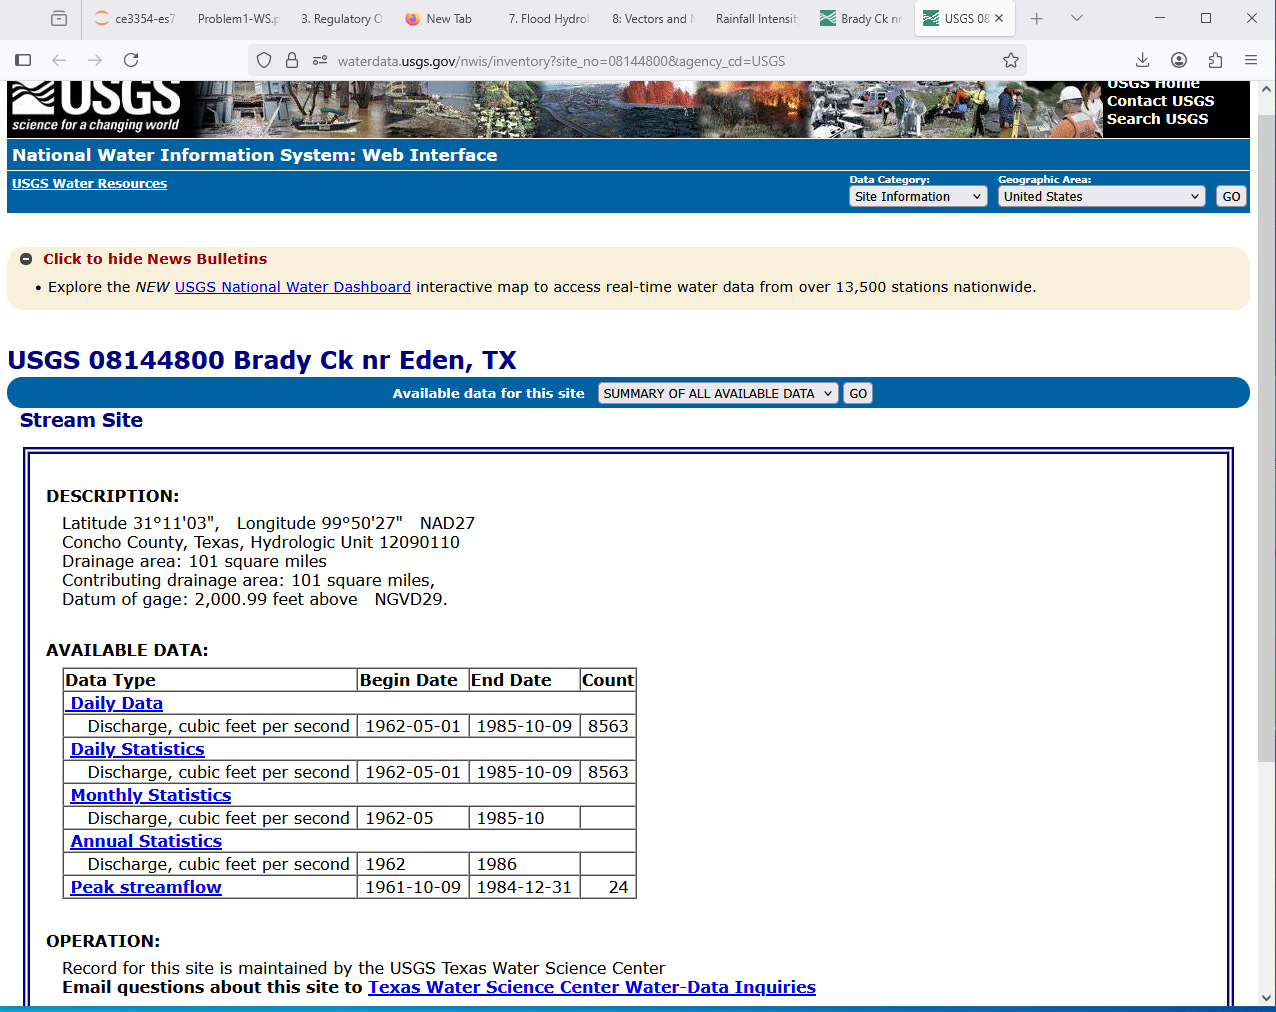
\includegraphics[width=7in]{nwis-inventory.png} 
   \caption{NWIS Inventory Page for 08144800, choose peak streamflow link}
   \label{fig:nwis-inventory}
\end{figure}

\begin{figure}[h!] %  figure placement: here, top, bottom, or page
   \centering
   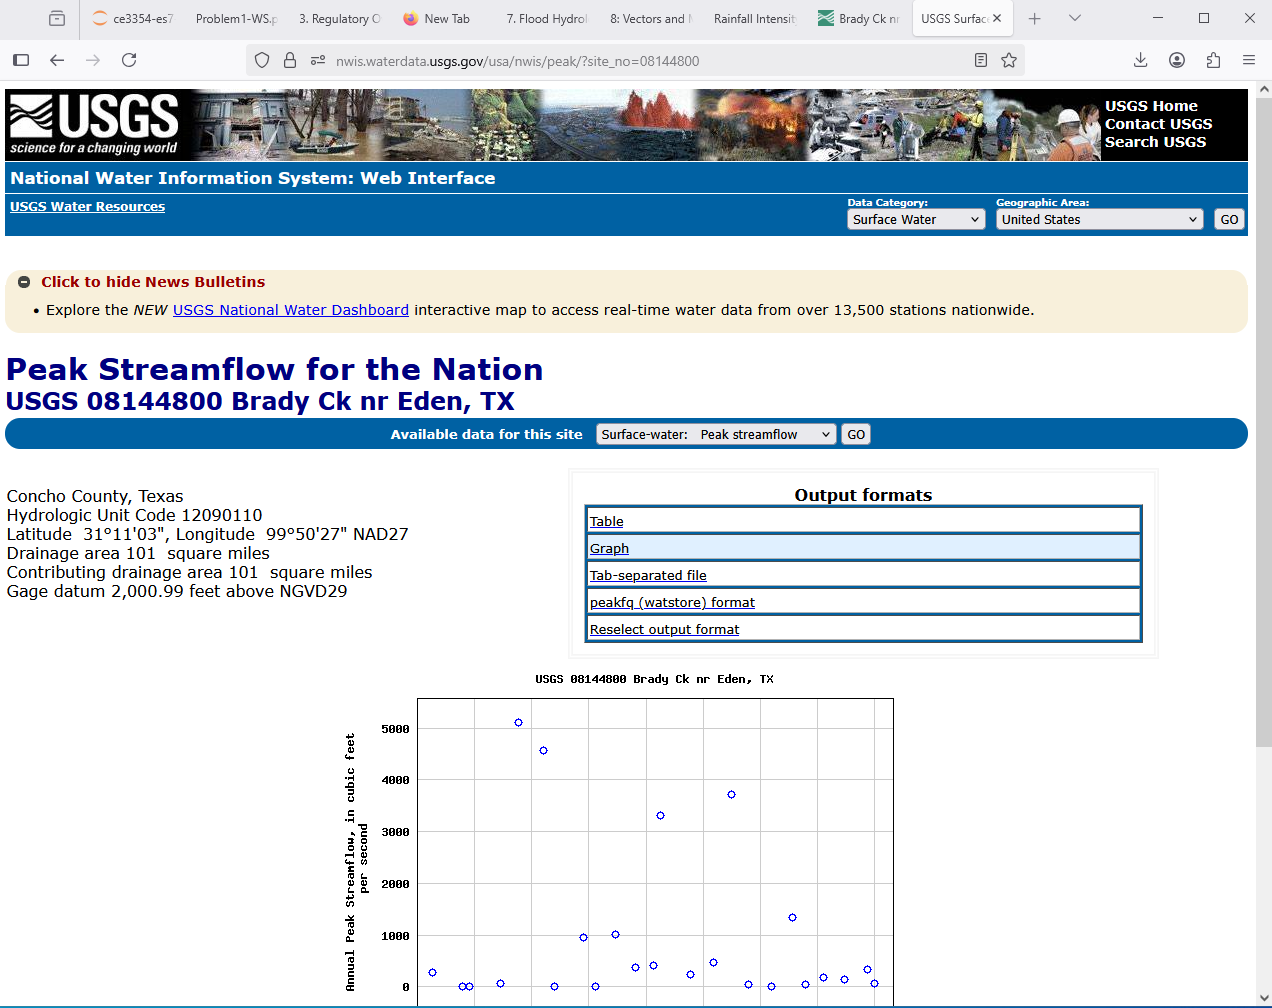
\includegraphics[width=7in]{DownloadPage.png} 
   \caption{Download Page for 08144800 (Note drainage area is shown here; about 101 square miles.}
   \label{fig:DownloadPage.png}
\end{figure}

\begin{figure}[h!] %  figure placement: here, top, bottom, or page
   \centering
   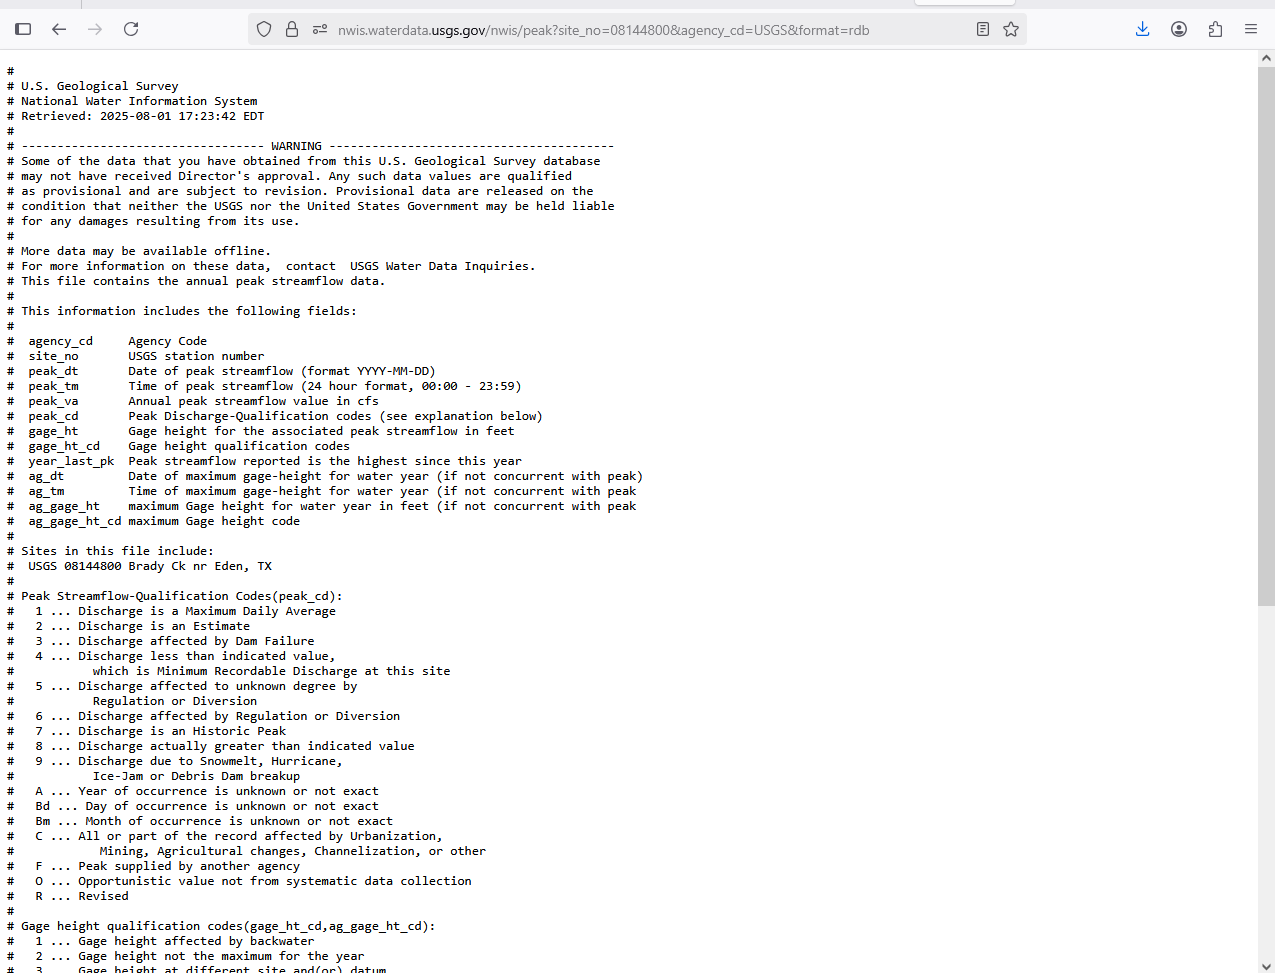
\includegraphics[width=7in]{brady-eden.png} 
   \caption{Data file excerpt - verify non-empty file}
   \label{fig:brady-eden}
\end{figure}

\begin{figure}[h!] %  figure placement: here, top, bottom, or page
   \centering
   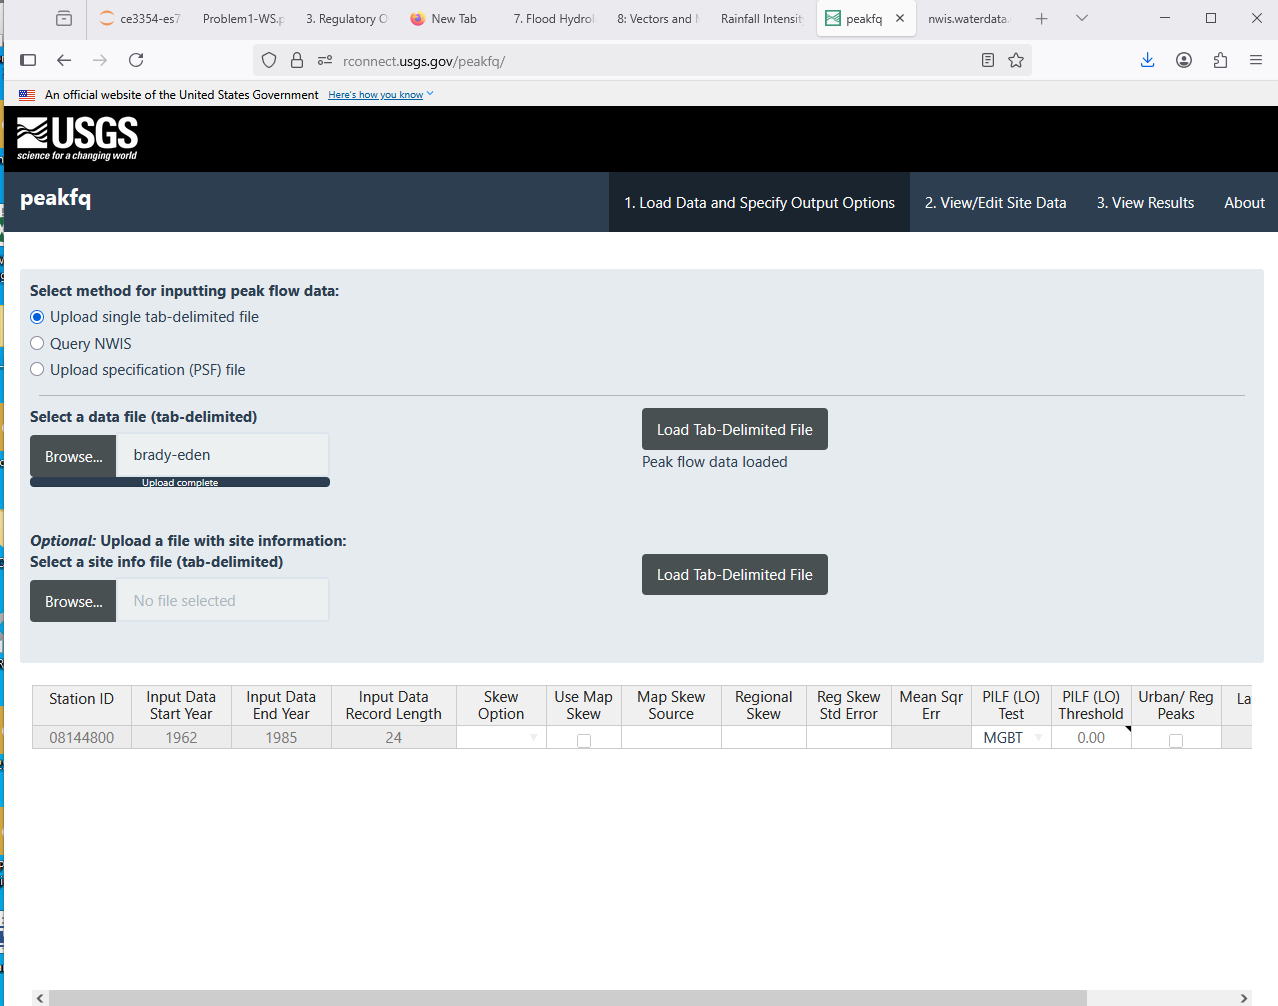
\includegraphics[width=7in]{peakfq-uploaded.png} 
   \caption{PeakFQ Landing Page - uploaded }
   \label{fig:peakfq-uploaded}
\end{figure}

\begin{figure}[h!] %  figure placement: here, top, bottom, or page
   \centering
   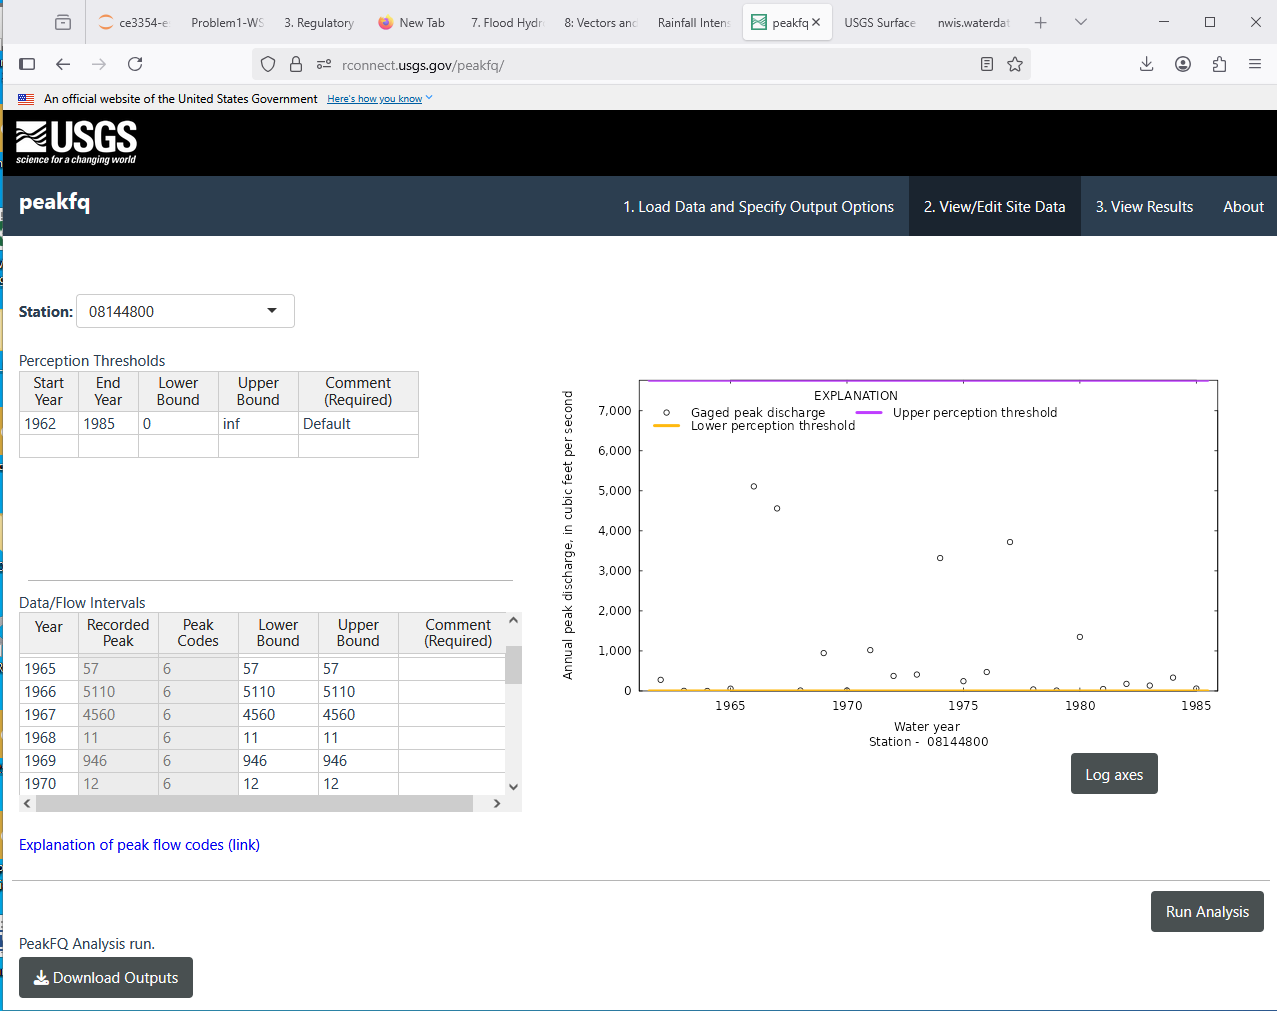
\includegraphics[width=7in]{peakfq-after-run.png} 
   \caption{PeakFQ run completed.  Had to select station skew and urban peaks}
   \label{fig:peakfq-after-run}
\end{figure}

\begin{figure}[h!] %  figure placement: here, top, bottom, or page
   \centering
   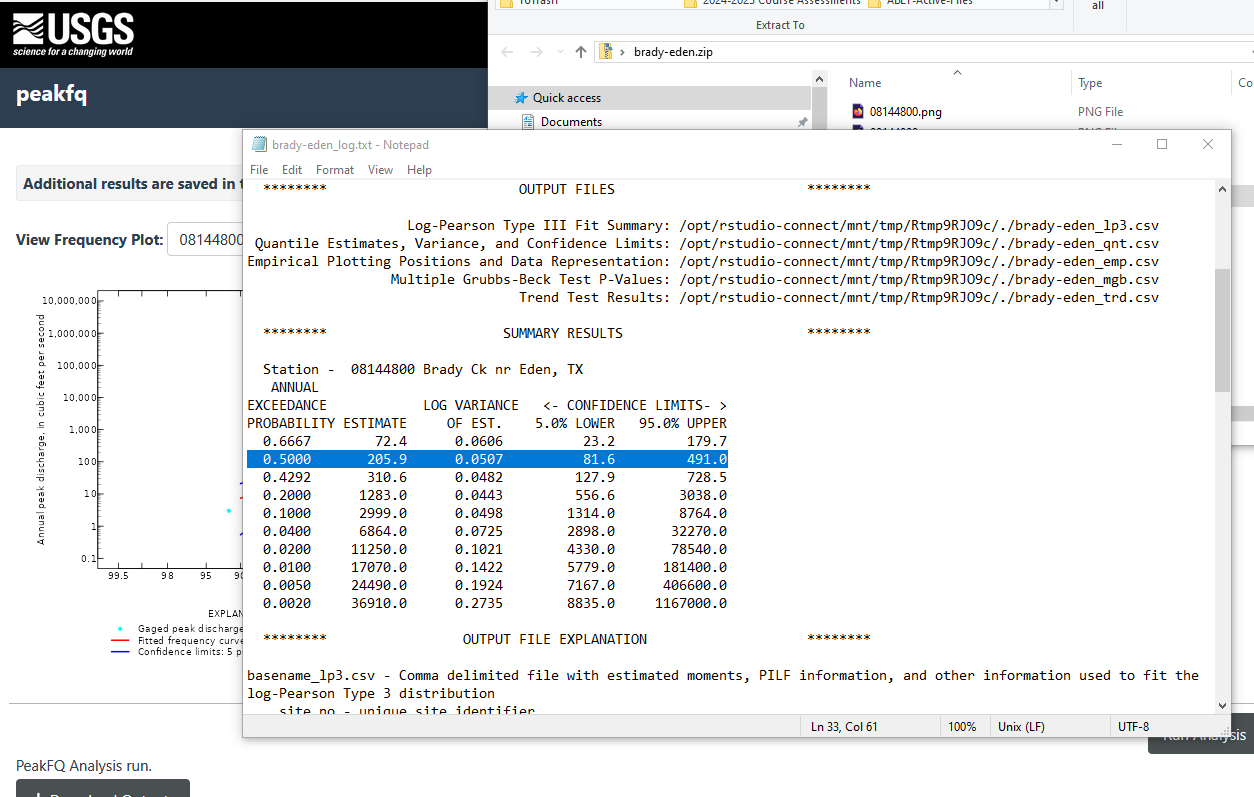
\includegraphics[width=7in]{output-table.png} 
   \caption{Tabulated output}
   \label{fig:output-table}
\end{figure}

\clearpage

From the tabulated output we can determine the discharge per square mile as

\begin{equation}
\frac{Q_{50\%}}{mi^2} = \frac{205.9~cfs}{101~mi^2} = 2.04 \frac{cfs}{mi^2}
\end{equation}

\end{enumerate}





\end{document}  